% vim: set spell spelllang=en tw=100 :

\documentclass[letterpaper]{article}

\setlength{\pdfpagewidth}{8.5in}
\setlength{\pdfpageheight}{11in}

\usepackage{aaai17}

\usepackage{times}
\usepackage{helvet}
\usepackage{courier}
\usepackage{complexity}
\usepackage{microtype}
\usepackage{amsmath}
\usepackage{amssymb}
\usepackage{amsthm}
\usepackage{cleveref}
\usepackage{tikz}
\usepackage{mathtools}
\usepackage{graphicx}
\usepackage{multicol}
\usepackage[ruled,vlined]{algorithm2e}

% to restate the propostions
\usepackage{thmtools,thm-restate}

\declaretheorem[name=Proposition,style=definition]{proposition}

\setcounter{secnumdepth}{2}

% \usepackage{showframe}

\makeatletter\@ifpackageloaded{showframe}{
    % show lines down the middle columns too
    % http://tex.stackexchange.com/questions/16199/test-if-a-package-or-package-option-is-loaded
\newlength\Fcolumnseprule\setlength\Fcolumnseprule{0.4pt}\def\@outputdblcol{%
  \if@firstcolumn\global \@firstcolumnfalse \global \setbox\@leftcolumn \box\@outputbox
  \else
    \global \@firstcolumntrue
    \setbox\@outputbox \vbox{\hb@xt@\textwidth{\hb@xt@\columnwidth{\box\@leftcolumn \hss}%
    \vrule \@width\Fcolumnseprule\hfil{\normalcolor\vrule \@width\columnseprule}
    \hfil\vrule \@width\Fcolumnseprule\hb@xt@\columnwidth {\box\@outputbox \hss}}}\@combinedblfloats\@outputpage
    \begingroup\@dblfloatplacement\@startdblcolumn\@whilesw\if@fcolmade \fi{\@outputpage\@startdblcolumn}\endgroup
  \fi
}}{}
\makeatother

\usetikzlibrary{decorations, decorations.pathreplacing, calc, backgrounds,shapes.misc}
%cross
\tikzset{cross/.style={cross out, draw=uofgcobalt, minimum size=2*(#1-\pgflinewidth), inner sep=0pt, outer sep=0pt},cross/.default={1.5mm}}


\definecolor{uofgsandstone}{rgb}{0.321569, 0.278431, 0.231373}
\definecolor{uofglawn}{rgb}{0.517647, 0.741176, 0}
\definecolor{uofgcobalt}{rgb}{0, 0.615686, 0.92549}
\definecolor{uofgpumpkin}{rgb}{1.0, 0.72549, 0.282353}
\definecolor{uofgthistle}{rgb}{0.584314, 0.070588, 0.447059}

\newcommand{\citet}[1]{\citeauthor{#1} \shortcite{#1}}
\newcommand{\citep}[1]{\cite{#1}}


\theoremstyle{definition}
\newtheorem{corollary}{Corollary}
\newtheorem{example}{Example}

% cref style
\crefname{figure}{Figure}{Figures}
\Crefname{figure}{Figure}{Figures}
\crefname{section}{Section}{Sections}
\Crefname{section}{Section}{Sections}
\crefname{proposition}{Proposition}{Propositions}
\Crefname{proposition}{Proposition}{Propositions}

\crefname{algocf}{Algorithm}{Algorithms}
\Crefname{algocf}{Algorithm}{Algorithms}

% http://tex.stackexchange.com/questions/22100/the-bar-and-overline-commands
\newcommand{\shortoverline}[1]{\mkern 1.5mu\overline{\mkern-1.5mu#1\mkern-1.5mu}\mkern 1.5mu}


% Maths operators
\newcommand{\paths}{\operatorname{paths}}
\newcommand{\lessnonind}[1]{\prescript{}{#1}{\rightarrowtail}\ }
\newcommand{\lessind}[1]{\prescript{}{#1}{\hookrightarrow}\ }
\newcommand{\lessmap}[1]{\prescript{}{#1}{\mapsto}\ }
\newcommand{\lesspreceq}[1]{\prescript{}{#1}{\preceq}\ }
\newcommand{\V}{\operatorname{V}}
\newcommand{\N}{\operatorname{N}}
\newcommand{\nds}{\operatorname{S}}
\newcommand{\loopcomp}[1]{\oset[.1ex]{\multimap}{#1}}

\makeatletter
\newcommand{\oset}[3][0ex]{%
  \mathrel{\mathop{#3}\limits^{
    \vbox to#1{\kern-2\ex@
    \hbox{$\scriptstyle#2$}\vss}}}}
\makeatother

\title{Between Subgraph Isomorphism and Maximum Common Subgraph}

\author{Anonymous \and Anonymous\thanks{This work was supported by an anonymous funding agency [grant number 12345]} \and Anonymous\thanks{This work was supported by an anonymous funding agency [grant number 67890]} \\
Top Secret Research Lab, Atlantis \\
anonymous@anonymous}

\pdfinfo{
    /Title (Between Subgraph Isomorphism and Maximum Common Subgraph)
    /Author (Anonymous and Anonymous and Anonymous)
}

\begin{document}

\maketitle

\begin{abstract}
    When a small pattern graph does not occur inside a larger target graph, we can ask how to find
    ``as much of the pattern as possible'' inside the target graph. In general, this is known as the maximum
    common subgraph problem, which is much more computationally challenging in practice than
    subgraph isomorphism. We introduce a restricted alternative, where we ask if all but $k$
    vertices from the pattern can be found in the target graph. This allows for the development of
    slightly weakened forms of certain invariants from subgraph isomorphism which are based upon degree and
    number of paths.  We show that when $k$ is small, weakening the invariants still retains much of
    their effectiveness. We are then able to solve this problem on the standard problem
    instances used to benchmark subgraph isomorphism algorithms, despite these instances being
    too large for current maximum common subgraph algorithms to handle. Finally, by iteratively
    increasing $k$, we obtain an algorithm which is also competitive for the maximum common subgraph
    problem.
\end{abstract}

\section{Introduction}

The subgraph isomorphism problem is to find a copy of a small \emph{pattern} graph inside a larger
\emph{target} graph. This is used in many areas, including bioinformatics \citep{Bonnici:2013},
computer vision \citep{cviu11,pr15}, malware detection \citep{DBLP:conf/dimva/BruschiMM06},
compilers \citep{DBLP:conf/cgo/MurrayF12,DBLP:conf/cp/BlindellLCS15}, and pattern recognition
\citep{Conte:2004}.  The problem comes in two forms: in the non-induced variant, edges must be
mapped to edges, but the target may have ``extra edges'', whilst in the induced variant, non-edges
may only be mapped to non-edges.

When a pattern cannot be found, we may wish to be given a result which maps as many vertices of the
pattern into the target as possible. In the induced case, this is known as the maximum common
induced subgraph problem (we discuss the non-induced case in \cref{section:definitions}). However,
although recent subgraph isomorphism algorithms are comfortable working with graphs with thousands
of vertices, the state of the art for the maximum common subgraph problem
\citep{DBLP:conf/cp/McCreeshNPS16} becomes computationally infeasible at only 35 vertices when
working with unlabelled graphs. This is largely because strong inference, based upon the degrees of
vertices \citep{DBLP:journals/ai/Solnon10} and the distances or paths between them
\citep{DBLP:conf/cp/AudemardLMGP14,DBLP:conf/cp/McCreeshP15}, is possible with subgraph isomorphism,
but not maximum common subgraph, and so the state space in the former is much more restricted,
whilst filtering during search is vastly stronger.

In this work we discuss an intermediate problem, where we must map all but $k$ vertices of the
pattern graph into the target---we show an example in \cref{fig:subgraphexample}. (This in some
ways resembles the approximate subgraph matching model of \citet{DBLP:conf/cp/ZampelliDD05},
although we allow any vertex to be removed.) We show that if $k$ is reasonably small (say, between 1
and 5), then weakened forms of degree and path based filterings are still effective in pruning the
initial search space and in providing additional constraints respectively. We then show that
combining these techniques leads to a practical algorithm which can scale to work with the families
of graphs commonly used to benchmark subgraph isomorphism algorithms: depending upon the benchmark
family, we can close a substantial portion of the instances, and in many more cases, we can at least
obtain an upper bound. This is a significant improvement over state of the art maximum common
subgraph solvers, which cannot even fit many of these instances in RAM. Finally, we show that
iteratively increasing $k$ gives a competitive algorithm for the maximum common induced subgraph
problem.

\begin{figure}
    \centering
    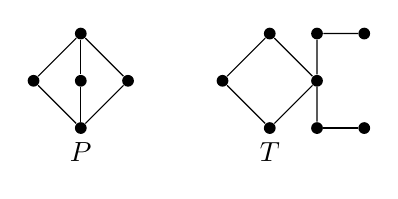
\begin{tikzpicture}[scale=0.6]%[every node/.style={circle, inner sep=0.5mm,node
        %distance=10mm,fill=black}, scale=0.2]

        \begin{scope}[xshift=-1cm, yshift=-3cm, color=black]
        \node at (0, -0.5) {$P$};
        \node [fill, circle, inner sep=1.5pt] (a) at (0,0) {};
        \node [fill, circle, inner sep=1.5pt] (b) at (-1,1) {};
        \node [fill, circle, inner sep=1.5pt] (c) at (0,1) {};
        \node [fill, circle, inner sep=1.5pt] (d) at (1,1) {};
        \node [fill, circle, inner sep=1.5pt] (e) at (0,2) {};

        \path[solid] (a) edge (b) edge (c) edge (d)
            (e) edge (b) edge (c) edge (d);
        % \node (a2) [below left of = aa,node distance=13mm,xshift=2mm] {};
        % \node (aa2) [above left of = a2,node distance=13mm,xshift=-2mm] {};
        % \node (ab2) [below left of = a2,node distance=13mm,xshift=-2mm] {};
        % \node (ac2) [fill=gray!50,above left of = ab2,node distance=13mm,xshift=-2mm] {};
        % \node (b2) [below right of = aa,node distance=13mm,xshift=-2mm] {};
        % \node (ba2) [above right of = b2,node distance=13mm,xshift=2mm] {};
        % \node (bb2) [below right of = b2,node distance=13mm,xshift=2mm] {};
        % \node (bc2) [fill=gray!50,above right of = bb2,node distance=13mm,xshift=2mm] {};

        % \node (aaa) [below of =aa, node distance=20mm] {};
        %
        % \path[dotted] (a) edge (a1) edge (b1);
        % \path (aa) edge (a1) edge (b1) edge (a2) edge (b2)
        %     (a1) edge (b1)
        %     (aaa) edge (a2) edge (b2)
        %     (a2) edge (aa2) edge (ab2)
        %     (b2) edge (ba2) edge (bb2);
        % \path[color=gray!50] (ac2) edge (ab2) edge (aa2)
        %     (bc2) edge (bb2) edge (ba2);
        %
        % \node [cross] {};
        \end{scope}

        \begin{scope}[xshift=3cm, yshift=-3cm, color=black]
        \node at (0, -0.5) {$T$};
        \node [fill, circle, inner sep=1.5pt] (a) at (0,0) {};
        \node [fill, circle, inner sep=1.5pt] (b) at (-1,1) {};
        \node [fill, circle, inner sep=1.5pt] (c) at (1,2) {};
        \node [fill, circle, inner sep=1.5pt] (d) at (1,1) {};
        \node [fill, circle, inner sep=1.5pt] (e) at (0,2) {};
        \node [fill, circle, inner sep=1.5pt] (f) at (1,0) {};
        \node [fill, circle, inner sep=1.5pt] (g) at (2,0) {};
        \node [fill, circle, inner sep=1.5pt] (h) at (2,2) {};

        \path[solid] (a) edge (b) edge (d)
            (e) edge (b) edge (d)
            (d) edge (c) edge (f)
            (c) edge (h)
            (f) edge (g);

        % \node (a2) [below left of = aa,node distance=13mm,xshift=2mm] {};
        % \node (aa2) [above left of = a2,node distance=13mm,xshift=-2mm] {};
        % \node (ab2) [below left of = a2,node distance=13mm,xshift=-2mm] {};
        % \node (ac2) [fill=gray!50,above left of = ab2,node distance=13mm,xshift=-2mm] {};
        % \node (b2) [below right of = aa,node distance=13mm,xshift=-2mm] {};
        % \node (ba2) [above right of = b2,node distance=13mm,xshift=2mm] {};
        % \node (bb2) [below right of = b2,node distance=13mm,xshift=2mm] {};
        % \node (bc2) [fill=gray!50,above right of = bb2,node distance=13mm,xshift=2mm] {};

        % \node (aaa) [below of =aa, node distance=20mm] {};
        %
        % \path[dotted] (a) edge (a1) edge (b1);
        % \path (aa) edge (a1) edge (b1) edge (a2) edge (b2)
        %     (a1) edge (b1)
        %     (aaa) edge (a2) edge (b2)
        %     (a2) edge (aa2) edge (ab2)
        %     (b2) edge (ba2) edge (bb2);
        % \path[color=gray!50] (ac2) edge (ab2) edge (aa2)
        %     (bc2) edge (bb2) edge (ba2);
        %
        % \node [cross] {};
        \end{scope}

    \end{tikzpicture}
    \caption{The pattern graph $P$ on the left cannot be found in the target graph $T$, but if
    the central vertex in the diamond is removed, then a subgraph isomorphism exists.}
    \label{fig:subgraphexample}
\end{figure}
\subsection{Definitions and Notations} \label{section:definitions}

A non-induced subgraph isomorphism from a graph $P$ to a graph $T$ is an injective mapping $P
\rightarrowtail T $ which maps adjacent vertices to adjacent vertices. An induced subgraph
isomorphism $P \hookrightarrow T$ additionally maps non-adjacent vertices to non-adjacent vertices.
We define a $k$-less subgraph isomorphism from $P$ to $T$ to be a subgraph isomorphism from all but
$k$ vertices of $P$ to $T$; this may be non-induced or induced, written $P \lessnonind{k} T$ and $P
\lessind{k} T$ respectively.

The \emph{complement} of a (simple) graph $P$ is the graph $\shortoverline{P}~$.  Adjacent distinct
vertices in $P$ are non-adjacent in $\shortoverline{P}$ while non-adjacent vertices in $P$ are
adjacent in $\shortoverline{P}$.  The \emph{loop complement} of a graph $P$ is the graph
$\loopcomp{P}$.  The construction of $\loopcomp{P}$ is similar to that of $\bar{P}~$, however
whenever a vertex has a loop in $P$ it does not in $\loopcomp{P}$ and vice versa.  When solving an
induced subgraph isomorphism problem we make use of the loop complement; we care about mapping
vertices with loops to vertices with loops, and vertices without loops to vertices without loops.
The following proposition follows directly from the definitions.

\begin{proposition}
    \label{prop:comp}
Let $i$ be an assignment of $T$ vertices to $P$ vertices.  Then $i$ satisfies the definition of $P
\hookrightarrow T$ if and only if $i$ satisfies $P \rightarrowtail T$ and
$\loopcomp{P} \rightarrowtail \loopcomp{T}$.
Similarly, $i$ satisfies the definition of $P
\lessind{k} T$ if and only if $i$ satisfies both $P \lessnonind{k} T$ and
$\loopcomp{P}
\lessnonind{k} \loopcomp{T}$.
\end{proposition}

A \emph{common induced subgraph} of graphs $G$ and $H$ is a graph $P$, together with two induced subgraph
isomorphisms to $G$ and $H$; a \emph{maximum common induced subgraph} is a common induced subgraph with as
many vertices as possible. An induced $k$-less subgraph isomorphism $P \lessind{k} T$ is equivalent
to a common induced subgraph of $P$ and $T$ with $\left|\V(P)\right| - k$ vertices.

If defined similarly, a maximum common non-induced subgraph would allow us to select every vertex in
the smaller of the two graphs, and none of the edges. It is therefore traditional to change the
objective to maximise the number of edges selected, rather than vertices, when a non-induced common
subgraph is sought---this problem is usually called the maximum common \emph{partial} subgraph
problem instead \citep{DBLP:conf/cp/NdiayeS11}. However, this is not what we will be discussing in
this paper: maximum common subgraph problems are symmetric in their inputs, but when discussing the
non-induced case we are allowing extra edges only in the target graph, not in the pattern.

\subsection{Constraint Models and Algorithms}

For both subgraph isomorphism and maximum common subgraph, constraint programming is the best known
approach\footnote{Note that toolkits are not used in state of the art implementations, to facilitate
better memory layouts and propagation queues, although the algorithms are heavily inspired by
constraint programming.}, although a reduction to maximum clique is better when edge labels are
present \citep{DBLP:conf/cp/NdiayeS11,DBLP:conf/cp/McCreeshNPS16}. For both problems, we create a variable for each vertex
in the pattern graph (the smaller graph, in the case of maximum common subgraph), with domains
ranging over the vertices in the target graph (the larger graph). For maximum common subgraph, each
domain is given an additional $\bot$ value, meaning ``unmapped''.

Constraints are used to ensure that adjacent pairs of vertices are mapped to adjacenct pairs of
vertices. For the maximum common subgraph case, any pair of assignments with $\bot$ as either value
is also permitted.  To handle the induced case, rather than the usual approach of directly
having constraints for non-adjacent pairs of vertices, we will make use of \cref{prop:comp} by
seeking a mapping $i$ which simultaneously satisfies $P \rightarrowtail T$ and $\loopcomp{P}
\rightarrowtail \loopcomp{T}$. Finally, an ``all different except $\bot$ constraint'' ensures
injectivity.

For subgraph isomorphism, this model can be enhanced with domain filtering at the top of search, to
reduce the initial sizes of domains---we discuss this in \cref{section:degreefiltering}. Subgraph
isomorphism also allows us to generate additional implied constraints, which we discuss in
\cref{section:pathfiltering}. However, neither of these techniques are valid for the maximum common
subgraph problem.

There are three easy ways we might try to extend existing algorithms for this problem.
A non-induced $k$-less subgraph isomorphism from $P$ to $T$ is equivalent to a subgraph isomorphism
between $P$ and $T$, with $k$ extra universally-adjacent vertices added to $T$, and so we could try
solving subgraph isomorphism with a modified target graph. However, using such
an approach is not ideal, because it would introduce symmetries; for induced $k$-less subgraph
isomorphisms, an approach based around adding vertices to $T$ cannot work at all.
Another algorithmic approach could be to try each way of removing $k$ vertices from the pattern
graph, and solving each subgraph isomorphism problem in turn. This approach might be feasible for $k
= 1$, although it would involve a lot of duplication of search effort, but for larger values of $k$
the number of searches which would have to be made would grow very quickly.
Finally, for the induced case we could try adapting maximum common subgraph algorithms to solve the
decision problem. However, both the maximum common subgraph algorithm and the clique encoding
require $O(\left|\V(P)\right|^2\left|\V(T)\right|^2)$ memory \citep{DBLP:conf/cp/McCreeshNPS16},
which is extremely problematic on the instances we wish to work with.

Instead, this paper introduces a new algorithm, inspired by a state of the art subgraph isomorphism
algorithm \citep{DBLP:conf/cp/McCreeshP15}. The approach we discuss requires only
$O(\left|\V(P)\right|^2\left|\V(T)\right|)$ space (this can be thousands of times less than maximum
common subgraph approaches, once the constant factors and orders of $T$ in our instances are
considered).

\subsection{Experimental Setup} \label{section:setup}

We perform our experiments on systems with dual Intel Xeon CPU E5-2640 processors with 64GBytes of
RAM, running Ubuntu 14.04. Our algorithm was implemented in C++\footnote{URL removed for anonymous
review}, and source code was compiled using
GCC 5.3.0. We used a timeout of 1,000 seconds for each instance. For comparison, we used the
implementations of \citet{DBLP:conf/cp/McCreeshNPS16}.

For datasets, we use the same 5,725 instances used in a recent work on portfolios of algorithms for
subgraph isomorphism \citep{thelionpaper}. This collection includes randomly generated scale-free
graphs \citep{constraints10}, an assortment of real-world graphs of varying sizes \citep{LV02},
randomly generated graph pairs (using bounded degree, regular mesh, and uniform models; all are
satisfiable), segmented images~\citep{pr15,cviu11}, meshes from modelling 3D objects \citep{cviu11},
and graphs close to the satisfiable-unsatisfiable phase transition
\citep{DBLP:conf/ijcai/McCreeshPT16}. All of these instances are available in a simple text
format\footnote{\texttt{http://liris.cnrs.fr/csolnon/SIP.html}}.  Note that many of these instances
are \emph{much} larger than were used in the recent comparison of maximum common subgraph algorithms
by \citet{DBLP:conf/cp/McCreeshNPS16}: for unlabelled graphs, they used pairs of graphs with up to
35 vertices in each, whilst our dataset contains graphs with up to 6,671 vertices. For the CP
algorithm, 1,560 of the instances cannot fit in the amount of RAM we have available---we treat these
instances as having timed out. The situation for the clique encoding is even worse, and 3,653 of
these instances do not fit in 64GBytes of RAM. In contrast, for our algorithm, every instance fits
comfortably.  \section{Domain Filtering using Degrees}\label{section:degreefiltering}

Let $p$ be a vertex in a graph $P$. The \emph{degree} of $p$, $\deg(p)$, is the number of vertices
to which it is adjacent. The degree of vertices gives us an invariant, which may be used to
eliminate some infeasible values from domains.

\begin{figure}[t]
    \centering
    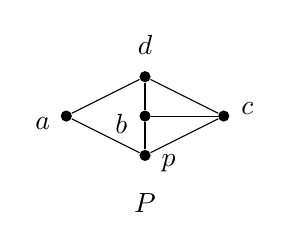
\begin{tikzpicture}[every node/.style={circle, inner sep=0.5mm}]
        \node[fill=black] (p) {};
        \node[fill=black] (b) [above of = p,node distance=5mm] {};
        \node[fill=black] (a) [left of = b] {};
        \node[fill=black] (c) [right of = b] {};
        \node[fill=black] (d) [above of = b,node distance=5mm] {};

        \node[draw=none,right of = p,node distance=3mm,yshift=-1mm] {$p$};
        \node[draw=none,left of = a,node distance=3mm,yshift=-1mm] {$a$};
        \node[draw=none,left of = b,node distance=3mm,yshift=-1mm] {$b$};
        \node[draw=none,right of = c,node distance=3mm,yshift= 1mm] {$c$};
        \node[draw=none,above of = d,node distance=3mm,yshift=1mm] {$d$};

        \node[draw=none, below of = p, node distance=6mm] {$P$};

        \path (p) edge (a) edge (b) edge (c)
            (a) edge (d)
            (b) edge (c) edge (d)
            (c) edge (d);
        \end{tikzpicture}\hspace{0.5cm}\begin{tikzpicture}[every node/.style={circle, inner sep=0.5mm}]
        \node[fill=gray!50] (a1) [right of = d, node distance = 2cm] {};
        \node[fill=black] (b1) [right of = a1] {};
        \node[fill=gray!50] (c1) [right of = b1] {};
        \node[fill=black] (a2) [below of = a1, node distance=6mm] {};
        \node[fill=black] (b2) [right of = a2] {};
        \node[fill=black] (c2) [right of = b2] {};
        \node[fill=gray!50] (a3) [below of = a2, node distance=6mm] {};
        \node[fill=black] (b3) [right of = a3] {};
        \node[fill=gray!50] (c3) [right of = b3] {};

        \node[draw=none,right of = b3,node distance=1mm, yshift=-2mm] {$q$};

        \node[draw=none, below of = b3, node distance=6mm] {$T$};

        \path[color=gray!50] (a1) edge (b1) edge (a2)
            (b1) edge (c1)
            (c1) edge (c2)
            (a2) edge (b2) edge (a3)
            (c2) edge (c3)
            (a3) edge (b3)
            (b3) edge (c3);
        \path[line width=0.4mm] (b1) edge (a2) edge (b2) edge (c2)
            (a2) edge (b3)
            (b2) edge (c2) edge (b3)
            (c2) edge (b3);
    \end{tikzpicture}\hspace{0.5cm}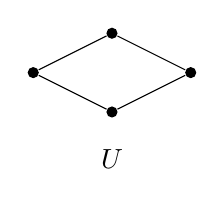
\begin{tikzpicture}[every node/.style={circle, inner sep=0.5mm}]
        \node[fill=black] (p) {};
        \node[draw=none] (b) [above of = p,node distance=5mm] {};
        \node[fill=black] (a) [left of = b] {};
        \node[fill=black] (c) [right of = b] {};
        \node[fill=black] (d) [above of = b,node distance=5mm] {};

        \node[draw=none, below of = p, node distance=6mm] {$U$};

        \path (p) edge (a) edge (c)
            (a) edge (d)
            (c) edge (d);
    \end{tikzpicture}
    \caption{There is a non-induced isomorphism $P\rightarrowtail T$ from the first graph to the
    second, using the highlighted vertices. No such isomorphism exists to the third graph, but there
    is a $1$-less isomorphism $P\lessnonind{1} U$ omitting vertex $b$.}\label{fig:klessexample}
\end{figure}

\begin{restatable}{proposition}{propdeg}\label{prop:deg}
    Let $p$ be a vertex in $P$ and $t$ a vertex in $T$. For both non-induced and induced
    $k$-less subgraph isomorphisms, if $p \lessmap{k} t$ then
    $\deg(p) - k \le \deg(t)$.
\end{restatable}

A vertex $q$ which is adjacent to $p$ is called its \emph{neighbour}.  Let $\N(p) = \{ q \in \V(P) :
 p~\textnormal{and}~q~\textnormal{are adjacent}\}$ be the set of neighbours of $p$.  The \emph{neighbourhood
degree sequence} (NDS) of $p$, $\nds(p)$, is the (non-ascending) sequence of degrees of its
neighbours.

Let $S = ( s_1 , \ldots , s_n )$ and $T = ( t_1 , \ldots , t_m)$ be two sequences.  We say that $S
\preceq T$ if $n \leq m$ and $\forall s_i \in S$ there exists a distinct $t_j \in T$ with $s_i \leq
t_j$.  When considering a $k$-less subgraph isomorphism we say that $S \lesspreceq{k} T$ if $n - k
\leq m$, and if there exists some subsequence $S_k$ of $S$ containing up to $k$ members such that
$\forall s_i \in S \setminus S_k$, there exists a distinct $t_j \in T$ with $s_i - k \leq t_j$.

\begin{restatable}{proposition}{propnds}\label{prop:nds}
If $p \lessmap{k} t$, then $\nds(p) \lesspreceq{k} \nds(t)$.
\end{restatable}

\begin{example}
Consider the pattern graph $P$ and the two target graphs $T$ and $U$ shown in
\cref{fig:klessexample}. The neighbourhood degree sequence of pattern vertex $p$ is
$\nds(p)=(3,3,2)$.
We highlight a subgraph in $T$ which is non-induced isomorphic to $P$. The vertex $p$ can be
mapped to $q$ in the target graph $T$, as $\nds(q)=(5,5,4,2,2)$.  There is a non-induced
mapping of the pattern graph $P$ into $U$ by removing $b$ of $P$.  This removal
changes the neighbourhood degree sequence of $p$ in the $k$-less version of $P$ to $\nds(p)=(2,2)$.
\end{example}

\Cref{fig:klessexample} also illustrates the three cases possible when filtering by neighbourhood degree
sequence.  Removing the top node causes each entry in $\nds(p)$ to be reduced; removing the
left-middle node removes an entry from $\nds(p)$; and removing either of the connected nodes in the
middle layer causes both the size of $\nds(p)$ to be reduced and an entry in $\nds(p)$ to be reduced.

\begin{corollary}
Since both $\nds(p)$ and $\nds(t)$ are non-ascending, without loss of generality we can replace
$S \setminus S_k$ from the definition of $S \lesspreceq{k} T$ with the subsequence consisting of all
    but the first $k$ members of $S$.
\end{corollary}

\begin{figure}
    \centering
    \includegraphics*{gen-graph-ids.pdf}
    \caption{The amount of domain reduction achieved for the induced problem, with increasing
    $k$. The $y$ value shows for how many instances we may reduce the initial search space to be
    at most the $x$ proportion of the size the search space would be for the maximum common subgraph
    problem.}\label{figure:ids}
\end{figure}

\Cref{figure:ids} demonstrates that this is effective in practice: we show the amount of domain
reduction we can achieve at the top of search by using invariants and a fixed $k$, compared to the
search space size for the maximum common induced subgraph problem. (The results on the non-induced
version show a similar but slightly weaker trend.)

Some other invariants do not translate. For example, another rule which can be effective on regular
graphs involves counting the number of neighbours of a vertex which are present in a triangle
\citep{mckay2014practical}. Removing a single vertex can alter this count arbitrarily, so we cannot
make use of this fact.

\begin{figure*}[t]
    \centering
    \includegraphics*{gen-graph-constraints-induced-0.pdf}
    \includegraphics*{gen-graph-constraints-induced-1.pdf}
    \includegraphics*{gen-graph-constraints-induced-2.pdf}
    \includegraphics*{gen-graph-constraints-induced-3.pdf}
    \includegraphics*{gen-graph-constraints-induced-4.pdf}
    \includegraphics*{gen-graph-constraints-induced-5.pdf}

    \caption{For the induced problem, the proportion of pairs of assignments from the filtered
    domains which are not permitted simultaneously, without path constraints on the $x$-axis and
    with path constraints on the $y$-axis, for increasing values of $k$.}\label{figure:constraints}
\end{figure*}

\section{Filtering During Search Using Paths}\label{section:pathfiltering}

As well as reasoning about degrees, we can also reason about paths.  A \emph{path} between two
vertices $p$ and $q$ is a sequence of edges which can be traversed from $p$ to reach $q$. We define
$\paths(p,q,n)$ to be the number of paths of length $n$ between the vertices $p$ and $q$.

\begin{restatable}{proposition}{proppaths}\label{prop:paths}
    Let $p,q \in \V(P)$ and $t,u\in \V(T)$. If $p \lessmap{k} t$ and $q \lessmap{k} u$ then
     $\paths(p, q, 2) - k \le \paths(t, u, 2)$.
\end{restatable}

\begin{corollary}
    For a graph $G$, let $G^{n, \ell}$ be the graph with vertex set $\V(G)$. The
    vertices $p$ and $q$ in $G^{n, \ell}$ are adjacent if there are at least $n$ simple paths of
    length exactly $\ell$ between $p$ and $q$ in $G$. Then any $k$-less subgraph isomorphism
    $P \lessnonind{k} T$ induces a new $k$-less subgraph isomorphism
    $P^{n+k, 2}\lessnonind{k} T^{n, 2}$.
\end{corollary}

Unlike in conventional subgraph isomorphism, we cannot extend this filtering to look at paths of
length three: removing a single vertex can delete arbitrarily many such paths. We \emph{could}
instead count paths of any length which are vertex disjoint, although calculating this appears to be
too expensive to be beneficial in practice.

To allow for fast propagation, rather than calculating paths dynamically like
\citet{DBLP:conf/cp/AudemardLMGP14}, we follow the approach of \citet{DBLP:conf/cp/McCreeshP15} and
construct \emph{supplemental graphs}, and find a mapping which is simultaneously a non-induced subgraph
isomorphism between every supplemental graph pair. We use paths of length 2, looking at path counts
of 1, 2, and 3 in the target graph (and so counts of $1 + k$ up to $3 + k$ in the pattern).  We then
investigate whether this leads to new constraints being generated.

By an assignment, we mean considering mapping a pattern vertex $p$ to a target vertex $t$ (and not
$\bot$) which does not violate any loop constraints. An assignment pair is two assignments with
distinct $p$ and distinct $t$, which we say is permitted if it does not violate any adjacency
constraint. We define the permitted assignment pair ratio to be the proportion of assignment pairs
which are permitted.  Finally, in \cref{figure:constraints} we scatter plot the permitted assignment
pair ratio with and without supplemental graphs\footnote{Because of the large sizes of the domains,
we randomly sample one million pairs rather than considering every pair. In some cases, we have
nearly a thousand domains, each with nearly ten thousand values---a complete quadratic calculation
involving even a trivial arithmetic operation on this would take many hours.}.

For $k = 0$, we see many points above the $x-y$ diagonal, which shows that for many instances, we
are able to create a substantial number of new constraints at the top of search; on the other hand,
there are also points on the diagonal, which shows that sometimes this technique provides no
benefit. (Occasionally, points fall below the $x-y$ diagonal.  This is because the use of
neighbourhood degree sequence reasoning on supplemental graphs can also lead to increased domain
filtering, which could in turn eliminate a higher proportion of forbidden than permitted assignment
pairs.) For $k = 1$ and $k = 2$, the proportion of points above the diagonal diminishes, but we are
still able to create new constraints for many instances. By the time $k = 3$, most of the benefit is
disappearing---although sometimes we are still able to make a difference, and bear in mind that
sometimes adding just one new constrained pair can vastly reduce the search space.

\section{A New Algorithm}\label{section:algorithm}

\begin{algorithm*}[tb]
\DontPrintSemicolon
\begin{multicols}{2}
\nl $\FuncSty{klessSubgraphIsomorphism}$ (\\\hspace*{2em}Graph $\mathcal{P}$, Graph $\mathcal{T}$, Int $k$) $\rightarrow$ Bool \;
\nl \Begin{
    \nl \lIf{$\left|\V(\mathcal{P})\right| + k > \left|\V(\mathcal{T})\right|$}{$\KwSty{return}~\KwSty{false}$\label{line:enough}}
    \nl $L \gets \big[ (\mathcal{P},\ \mathcal{T}), (\loopcomp{\mathcal{P}},
        \loopcomp{\mathcal{T}}) \textnormal{~only if we want induced\label{line:comp}},$
        \\\hspace*{1.0em}$(\mathcal{P}^{1 + k,2},\ \mathcal{T}^{1,2}), (\mathcal{P}^{2 + k,2},\
    \mathcal{T}^{2,2}), (\mathcal{P}^{3 + k,2},\ \mathcal{T}^{3,2}) \big]$ \;
    \nl \ForEach{$v \in \V(\mathcal{P})$}{
        \nl $D_v \gets \V(\mathcal{T})$\;
        \nl \ForEach{$(P,\,T) \in L$}{
            \nl $D_v \gets \{ w \in D_v : $ \\
            \hspace*{4em}$v \sim_P v \Rightarrow w \sim_T w~\wedge$ \\
            \hspace*{4em}$\nds_P(v) \lesspreceq{k} \nds_T(w)\}$ \;
        }
        \nl $D_v \gets D_v \cup k~\textnormal{distinct wildcard values}$
    }
    \nl \lIf{\FuncSty{propagate}(L, D)}{$\KwSty{return}~\FuncSty{search}(L, D, k)$}
    \nl \lElse{$\KwSty{return}~\KwSty{false}$}
}
\bigskip
\nl $\FuncSty{search}$ (GraphPairs $L$, Domains $D$, Int $k$) $\rightarrow$ Bool \;
\nl \Begin{
    \nl \lIf{$D = \emptyset$}{$\KwSty{return}~\KwSty{true}$}
    \nl $D_v \gets \textnormal{the smallest domain in}~D$ \;
    \nl \ForEach {$v' \in D_v~\textnormal{ordered by static degree in}~\mathcal{T}$\label{line:parforeach}}{
        \nl \If{$v'$ \textnormal{is not the first wildcard we have tried\label{line:sym}}}{
            \nl \KwSty{continue} \;
        }
        \nl $D' \gets \FuncSty{clone}(D)$ \;
        \nl $D'_v \gets \{ v' \} $ \;
        \nl \If{\FuncSty{propagate}(L, D')}{
            \nl \If{$\FuncSty{search}(L, \{ D \in D' : \left|D\right| > 1 \}, k)$}{
                \nl $\KwSty{return}~\KwSty{true}$ \;
            }
        }
    }
}
\bigskip
\nl $\FuncSty{propagate}$ (GraphPairs $L$, Domains $D$) $\rightarrow$ Bool \;
\nl \Begin{
    \nl \While{\KwSty{true}}{
        \nl \If{\textnormal{no effectively-unit domains remain (treating all wildcard~values as a single
            value)\label{line:effect}}}{
            \nl \If{$\KwSty{not}~\FuncSty{allDifferent}(D)$}{
                \nl $\KwSty{return}~\KwSty{false}$ \;
            }
        }
        \nl \If{\textnormal{no effectively-unit domains remain}}{
            \nl $\KwSty{return}~\KwSty{true}$ \;
        }
        \nl $D_v \gets \textnormal{an effectively-unit domain from}~D$ \;
        \nl $v' \gets $ the single value in $D_v$, or an arbitrary wildcard~value if there is more
        than one \;
        \nl \ForEach{$D_w \in D \setminus \{ D_v \}$}{
            \nl $D_w \gets D_w \setminus \{ v' \}$ \label{line:removev} \;
            \nl \ForEach{$(P,\,T) \in L$}{
                \nl \If{$v \sim_P w$}{
                    \nl $D_w \gets D_w \cap \left(\N_T(v') \cup \textnormal{wildcards}\right)$
                }
            }
            \nl \lIf{$D_w = \emptyset$}{$\KwSty{return}~\KwSty{false}$}
        }
    }
}
\bigskip
\nl $\FuncSty{allDifferent}$ (Domains $D$) $\rightarrow$ Bool \;
\nl \Begin{
\nl $(H,\,A,\,n) \gets (\emptyset,\,\emptyset,\,0)$ \;
\nl \ForEach{$D_v \in D$ \textnormal{from smallest to largest\label{line:eachdomain}}}{
    \nl $D_v \gets D_v \setminus H$ \label{line:elimhall} \;
    \nl $(A,\,n) \gets (A \cup D_v,\,n + 1)$ \label{line:acc} \;
    \nl \lIf{$D_v = \emptyset~\KwSty{or}~\left|A\right| < n$}{$\KwSty{return}~\KwSty{false}$\label{line:failhall}}
    \nl \lIf{$\left|A\right| = n$}{$(H,\,A,\,n) \gets (H \cup A,\,\emptyset,\,0)$\label{line:hall}}
}
\nl $\KwSty{return}~\KwSty{true}$ \;
}
\end{multicols}
\vspace*{0.4cm}% bug in algorithm2e + multicol: incorrect space left above the vertical line
\caption{An algorithm for the $k$-less subgraph isomorphism problem.}
\label{algorithm:sip}
\end{algorithm*}

\Cref{algorithm:sip} integrates these techniques into a full algorithm. This is derived from an
algorithm due to \citet{DBLP:conf/cp/McCreeshP15}, which in a recent evaluation of using portfolios
of subgraph isomorphism algorithms was the single strongest solver portfolios \citep{thelionpaper}.
As well as the modifications to solve $k$-less and induced problems, we have made two
simplifications: we do not use conflict-directed backjumping, and we do not use iterated label
filtering to recalculate neighbourhood degree sequences if vertices are not present in any target
domain after construction---in preliminary experiments, these techniques were not beneficial for $k
> 0$. We also do not strip isolated vertices, as this is not a valid simplification in the induced
case.

To handle wildcards, we include $k$ additional $\bot$ values in domains, rather than a single value
which may be used $k$ times. These are treated as having degree zero, in an attempt to maximising
the expected number of solutions remaining during search \citep{DBLP:conf/ijcai/McCreeshPT16}. This
technique allows us to retain the bit-parallel all different propagator used in the original
algorithm. However, we must be careful to treat domains containing multiple wildcard values (which
we call ``effectively unit'') specially during unit propagation (line~\ref{line:effect}), and we
introduce a symmetry break (line~\ref{line:sym}) to try only a single wildcard value for each
variable.

To handle the induced case, we make use of \cref{prop:comp} (line~\ref{line:comp}). We also tested
using path reasoning on complement graphs, but this is expensive to calculate and provides little
benefit in practice on the instances we considered.

\section{Empirical Evaluation}\label{section:evaluation}

\begin{figure*}[tb]
    \centering
    \includegraphics*{gen-graph-runtimes.pdf}
    \caption{In the first two plots we show the cumulative number of instances solved over time, for the
        induced and non-induced problems, with different values of $k$. We also show the results of
        iteratively increasing $k$ until a solution is found, and in the induced case, the
        performance of two leading maximum common subgraph algorithms. In the third plot we show results
        comparing iteratively increasing $k$ with our algorithm to other approaches on maximum
        common induced subgraph instances.}\label{figure:runtimes}
\end{figure*}

\begin{figure}[h!]
    \centering
    \includegraphics*{gen-graph-which-k-by-family.pdf}
    \caption{The proportion of instances, in different families, which become satisfiable for
    increasing values of $k$. The ``larger'' instances are those where we can prove unsatisfiability for
    $k = 5$, whilst the gap between the top of the bar and the top of the graph is the fraction of
    instances where a timeout was reached for at least one value of $k$.}\label{figure:which-k}
\end{figure}

We now evaluate our algorithm and show that it is effective in practice, even on the larger subgraph
isomorphism instances. In the first two plots of \cref{figure:runtimes} we give cumulative
distributions for the induced and non-induced problems, with $k$ ranging from $0$ to $5$ (we
discuss the dotted lines in this plot below). The results are strong: with $k = 0$ we may solve
nearly every instance, whilst even at $k = 5$ we can solve over $4,000$ instances in both variants.

But are we learning anything about the results---that is, are there instances for which $k = 0$ is
unsatisfiable, but that are satisfiable for small $k$? For the problem families which do not consist
entirely of satisfiable instances, we plot this in \cref{figure:which-k}. In the ``phase'' family,
which consists of instances crafted to be extremely difficult to solve, we are not able to answer
this question, and in the ``scalefree'' family we see no satisfiable instances with low but not zero
$k$ (this is simply due to there being many vertices with loops in some pattern graphs, but no loops
at all in the targets). However, in several of the remaining families we can more than double the
number of instances for which exact solutions are known, and gain upper bounds on many more. This is
particularly interesting for the ``images-CVIU11'' family due to \citet{cviu11}, where the size of
the solution has a direct real-world interpretation in terms of closeness of image matching.

\subsection{Solving from the Top Down}

What would happen if we used our approach to solve the maximum common induced problem? We could
simply start at $k = 0$, and increase $k$ until a solution is found. This would be tackling the
problem in the opposite direction from existing approaches, which work by attempting to construct
larger and larger solutions. The dotted lines in \cref{figure:runtimes} show this approach: the $k
\downarrow$ is our algorithm, whilst ``FC'' and ``clique'' are the two algorithms discussed by
\citet{DBLP:conf/cp/McCreeshNPS16}.  Recalling the disclaimer in \cref{section:setup}
regarding instances not fitting in the 64GBytes of RAM we have available, we see that our approach is
able to close over twice as many of these instances as the previous state of the art. (The same
conclusion holds even if every instance which is satisfiable with $k = 0$ is removed from the
dataset.)

What about if we use instances designed for the maximum common subgraph problem? In the third plot
in \cref{figure:runtimes} we again compare these approaches, but using the first ten instances from
each family of a standard benchmark set
\citep{DBLP:journals/prl/SantoFSV03,DBLP:journals/jgaa/ConteFV07}, selecting undirected, unlabelled
graphs with up to 50 vertices---this gives us a total of 4,110 instances. In these instances the
number of vertices in the pattern and target graphs is the same, which is not ideal for our
algorithm (although our invariants are still effective in many cases). Nonetheless, we are by a
small margin the single strongest solver. Interestingly, our algorithm tends to have complementary
performance to the other two approaches (which are much more correlated), which suggests that there
is scope for an algorithm which runs both an upper bound and a constructive, lower bound approach
simultaneously or in parallel, stopping when the two bounds meet in the middle.

\section{Conclusion}

By considering a restricted variation of the problem, we have been able to go some of the way
towards tackling the maximum common subgraph problem on much larger graphs than have previously been
possible. We saw that some invariants from the subgraph isomorphism problem can still be used,
albeit in a weakened form, with considerable effect when a small number of vertices can be removed.
We have by no means cracked the problem completely---our results are still far from where we
would like them to be for use in real-world applications, and many instances remain open. However,
for many of the open instances we are at least able to get upper bounds on the result for the
first time.

In future work, we will combine this approach with existing lower bounding construction methods, to
deliver a hybrid algorithm. We also intend to allow restrictions on which vertices may or may not be
removed, similar to the approach of \citet{DBLP:conf/cp/ZampelliDD05}, but with much stronger
filtering now being possible.

% \section*{Acknowledgements}

\bibliographystyle{aaai}
\bibliography{paper}

\clearpage
\appendix

\section{Proofs Omitted From Main Text}

The following proofs have been omitted from the main text. If the reviewers feel they are helpful
and not obvious, we will pay for an extra page to include them.

\bigskip

\propdeg*
\begin{proof}
Let $p$ be a vertex in $P$, and $t$ a vertex in $T$, with $p\mapsto t$. Then by the definition of subgraph isomorphisms, $\deg(p) \le \deg(t)$. Let $P'$ be $P$ less $k$ vertices and $p$ a vertex in $P'$. Then
\[
\deg_{P}(p)-k \le \deg_{P'}(p) \le \deg_{P}(p) \le \deg(t). \qedhere
\]
\end{proof}

\bigskip

\propnds*
\begin{proof}
Let $p \lessmap{k} t$.  Then $\deg(p) - k \leq \deg(q)$, by \cref{prop:deg}, which
implies that $\left|\nds(p)\right| -k \leq \left| \nds(t) \right| $.

Also, $p \lessmap{k} t$ implies that for each $q \in N(p) \setminus P_k$, where $P_k$
is some subset of $P$ with $\left| P_k \right| \leq k$, we have $q \lessmap{k} u$, where $u \in N(t)$ and
each $u$ is distinct.  Then $\deg(q) - k \leq \deg(u)$, by \cref{prop:deg}.  Hence $\nds(p)
\lesspreceq{k} \nds(t)$.
\end{proof}

\bigskip

\proppaths*
\begin{proof}
Let $P_{2}$ be the set of all paths of length two between $p$ and $q$, \[P_{2} = \{((p,x),(x,q)) :
(p,x),(x,q)\in \operatorname{E}(P) \}\textnormal{.}\] As we are looking at paths of length 2,
the intermediate vertices lie in both neighbour vertex sets of $p$ and $q$. We can rewrite
$P_{2}$ as \[P_{2} = \{((p,x),(x,q)) : x\in \N(p) \text{ and } x\in \N(q) \}\textnormal{,}\] in
other words the intermediate vertices lie in the intersection of the neighbour sets of $p$ and
$q$, \[ P_{2}=\{((p,x),(x,q)) : x\in \N(p)\cap \N(q) \} \textnormal{.}\] Therefore
$\paths(p,q,2) = \left| \N(p)\cap \N(q) \right|  \leq \deg(p)$.

If we remove up to $k$ vertices from the neighbourhood of $p$, it will impact the intersection of
    the neighbourhoods of $p$ and $q$, and by Proposition~\ref{prop:deg}, as $p\lessmap{k}t$,
\[
\left| \N(p)\cap \N(q)\right| - k \leq \deg(p) - k \leq \deg(t).
\]
As $\left|\N(p)\cap \N(q)\right|\leq \deg(p) \leq \left|\N(t)\cap \N(u)\right|\leq \deg(t)$, we have
\begin{align*}
\left|\N(p)\cap \N(q)\right| - k & \leq \deg(p) - k \\
 & \leq \left|\N(t)\cap \N(u)\right|\\
 & \leq \deg(t)
\end{align*}
which tells us
\[
\paths(p, q, 2) - k \leq \paths(t, u, 2). \qedhere
\]
\end{proof}

\end{document}
